\documentclass[conference]{IEEEtran}

\IEEEoverridecommandlockouts

\usepackage{cite}
\usepackage{amsmath,amssymb,amsfonts}
\usepackage{algorithmic}
\usepackage{graphicx}
\usepackage{textcomp}
\usepackage{xcolor}
\usepackage{amsfonts}
\usepackage{tikz}
\usepackage{float}

\def\BibTeX{{\rm B\kern-.05em{\sc i\kern-.025em b}\kern-.08em
    T\kern-.1667em\lower.7ex\hbox{E}\kern-.125emX}}

\begin{document}

    \title{Reliable Tether Enclosing Using Interval Analysis}

    \author{\IEEEauthorblockN{Quentin Brateau} ENSTA Bretagne}

    \maketitle

    \begin{abstract}
        Remotely Operated Vehicles (ROV) are used in a a lot of fields in marine operations, such as
        underwater inspections. These robots are linked to operators using tether to get power and
        to communicate.
    \end{abstract}

    \begin{IEEEkeywords}
        Interval Analysis, Tether, Reliable, Sets Theory
    \end{IEEEkeywords}

    \section{Introduction}

    \section{Formalism}
        First we need to consider the problem in the plane $(O, x, z)$. Assuming that the tether is 
        bound at its extremities at $A (x_A, z_A)$ and $B (x_B, z_B)$ and that its length is $L$. 
        Considering a point $M (x, z)$ belonging to the boundary of the set enclosing the tether,
        we could have the following constrain :

        \begin{equation}
            d(A, M) + d(M, B) \leq L \\
        \end{equation}

        Where $d(A, M) = \sqrt{(x_M - x_A)^2 + (z_M - z_A)^2}$ is the euclidian distance between
        $A$ and $M$.

        \begin{figure}[H]
            \centering
            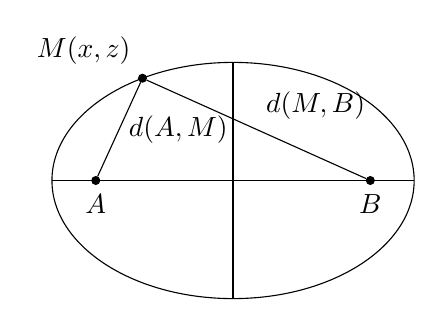
\begin{tikzpicture}[dot/.style={draw,fill,circle,inner sep=1pt}]
                \def\a{2.3} % large half axis
                \def\b{1.5} % small half axis
                \def\angle{120} % angle at which X is placed
                % Draw the ellipse
                \draw (0,0) ellipse ({\a} and {\b});
                % Draw the inner lines and labels
                \draw (-\a,0) -- (\a,0);
                \draw (0,-\b) -- (0,\b);
                % Nodes at the focal points
                \node[dot,label={below:$A$}] (F1) at ({-sqrt(\a*\a-\b*\b)},0) {};
                \node[dot,label={below:$B$}] (F2) at ({+sqrt(\a*\a-\b*\b)},0) {};
                % Node on the rim, connected to foci
                \node[dot,label={\angle:$M (x, z)$}] (X) at (\angle:{\a} and {\b}) {};
                \draw (F1) -- (X) node[midway, right] {$d(A, M)$} (X) -- (F2) node[midway, above right] {$d(M, B)$};
            \end{tikzpicture}
            \caption{Set bounding the tether}
        \end{figure}

        Then the tether is bounded in the set $\mathbb{T}$ representing an ellipse of foci $A$ and $B$ :

        \begin{equation}
            \mathbb{T} = \{(x, z) \in \mathbb{R} \mid d(A, M) + d(M, B) \leq L \}
        \end{equation}

\end{document}
